\section{O problema}

\begin{frame}{Problema inverso}

  \textbf{Objetivo:} estimar o vetor de parâmetros
  $\theta=(r,K,a,h,e,m)$ do modelo de Rosenzweig--MacArthur.

  \vspace{0.3cm}

  \begin{columns}[c,onlytextwidth]
    \begin{column}{0.53\textwidth}
      \[
        \left\{
        \begin{aligned}
          \dot N &= rN\left(1-\frac{N}{K}\right)
                    -\frac{aNP}{1+ahN}, \\[0.3cm]
          \dot P &= e\frac{aNP}{1+ahN}-mP.
        \end{aligned}
        \right.
      \]
    \end{column}
    \begin{column}{0.45\textwidth}
      \small
      \begin{itemize}
        \item $r$: taxa de crescimento das presas;
        \item $K$: capacidade de suporte;
        \item $a$: taxa de ataque;
        \item $h$: tempo de manipulação da presa;
        \item $e$: eficiência de conversão;
        \item $m$: taxa de mortalidade dos predadores.
      \end{itemize}
    \end{column}
  \end{columns}

  \vspace{0.3cm}

  A calibração é realizada a partir de observações das populações
  de presas $N(t)$ e predadores $P(t)$, com condições iniciais
  conhecidas.

  \[
    \hat{\theta}=\arg\min_{\theta\in\Theta} J(\theta),
  \]

  onde $\Theta$ representa o espaço admissível de parâmetros.

\end{frame}

\begin{frame}{Geração dos dados sintéticos}

  Os dados sintéticos são obtidos pela integração numérica do
  modelo de Rosenzweig-MacArthur pelo método RK45.

  \vspace{0.3cm}

  \begin{columns}[c,onlytextwidth]
    \begin{column}{0.32\textwidth}

      \centering
      \textbf{Parâmetros de referência}

      \begin{center}
        \begin{tabular}{c|c}
          \hline
          Parâmetro & Valor \\
          \hline
          $r$ & $1$ \\
          $K$ & $100$ \\
          $a$ & $0{,}05$ \\
          $h$ & $0{,}2$ \\
          $e$ & $0{,}5$ \\
          $m$ & $0{,}5$ \\
          \hline
        \end{tabular}
      \end{center}

    \end{column}

    \begin{column}{0.66\textwidth}
      \begin{figure}
        \centering
        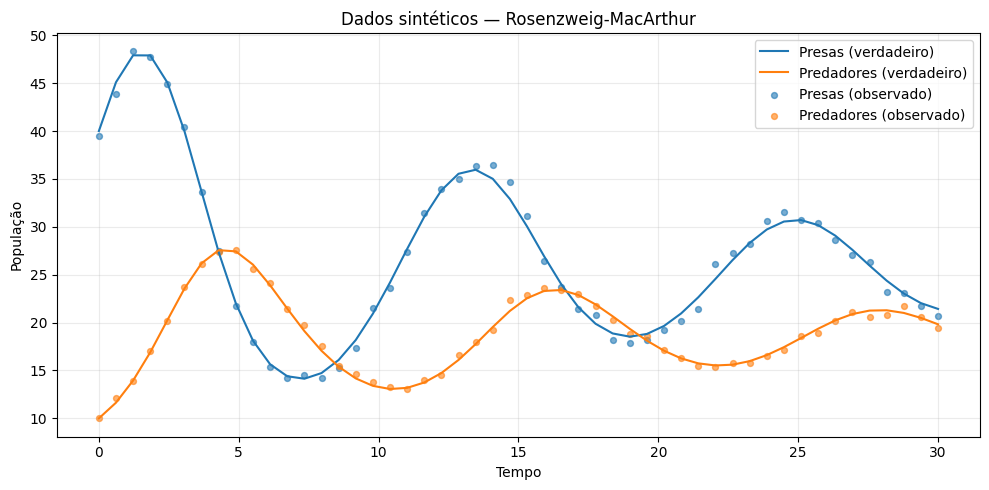
\includegraphics[width=\textwidth]{imgs/dados_atualizados.png}
        \caption{Dados sintéticos com ruído gaussiano de 2\%.}
      \end{figure}
    \end{column}
  \end{columns}

  \vspace{0.3cm}

  \begin{itemize}
    \item Condições iniciais: $N(0)=40$ e $P(0)=10$.
    \item 50 instantes de observação no intervalo $t\in[0,30]$.
  \end{itemize}

\end{frame}

\begin{frame}{Protocolo experimental}

  \textbf{Perturbação das observações:}

  \[
    X_i^{\mathrm{obs}}=X_{\theta^*}(t_i)+\varepsilon_i,
    \qquad
    \varepsilon_i\sim\mathcal{N}(0,\sigma_X^2),
  \]

  \[
    \sigma_X=\delta A_X^*,
    \qquad \delta\in\{0;\,0{,}02;\,0{,}05\},
  \]

  onde $X\in\{N,P\}$ e $A_X^*$ é a amplitude da
  trajetória original, sem ruído.

  \vspace{0.3cm}

  \textbf{Distribuição dos experimentos:}

  \begin{table}
    \centering
    \begin{tabular}{c|c|c|c}
      \hline
      Ruído & Realizações & AG por realização & Total \\
      \hline
      $0\%$ & 1 & 30 & 30 \\
      $2\%$ & 3 & 30 & 90 \\
      $5\%$ & 3 & 30 & 90 \\
      \hline
      \textbf{Total} & \textbf{7} & -- & \textbf{210} \\
      \hline
    \end{tabular}
  \end{table}

  O protocolo permite avaliar a influência do ruído nas
  observações e da natureza estocástica do algoritmo genético.

\end{frame}

\section{Metodologia}

\begin{frame}{Visão geral da calibração}

  \small
  Para cada realização dos dados observados, o algoritmo genético busca o vetor
  $\theta=(r,K,a,h,e,m)$ que minimiza a função objetivo $J(\theta)$.

  \vspace{0.35cm}

  \begin{figure}
    \centering
    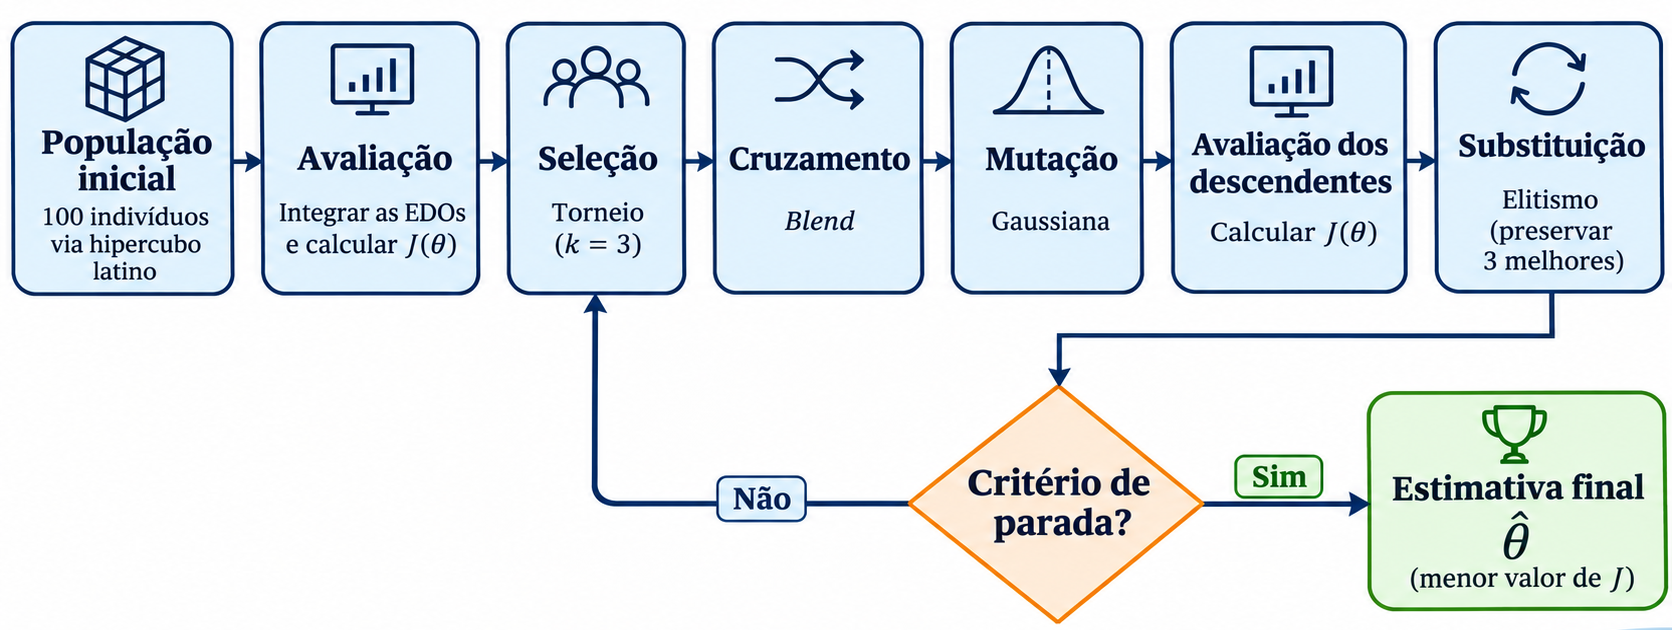
\includegraphics[width=0.85\textwidth]{imgs/overview.png}
    \caption{Visão geral do processo de calibração com algoritmo genético. Fonte: Imagem gerada pelo ChatGPT.}
  \end{figure}

\end{frame}

\begin{frame}{Inicialização da população}

  \begin{itemize}
    \item \textbf{Codificação real:} cada cromossomo representa
          um vetor de parâmetros $\theta_i\in\mathbb{R}^{6}$.

    \item \textbf{População inicial:} 100 indivíduos amostrados
          por hipercubo latino (LHS), favorecendo a diversidade
          e a exploração do espaço de busca.

    \item Cada dimensão do hipercubo unitário é dividida em
          100 estratos equiprováveis, amostrados uma única vez
          por coordenada.
  \end{itemize}

  O mapeamento para o domínio admissível é dado por:

  \[
    \theta_{ij}^{(0)}=L_j+u_{ij}(U_j-L_j),
    \qquad u_{ij}\in[0,1],
  \]

  onde $u_{ij}$ é obtido pela amostragem LHS.

  \begin{table}
    \centering
    \begin{tabular}{lrrrrrr}
      \toprule
      Parâmetro & $r$ & $K$ & $a$ & $h$ & $e$ & $m$ \\
      \midrule
      $L_j$ & $0{,}2$ & $40$ & $0{,}005$ & $0{,}02$ & $0{,}1$ & $0{,}05$ \\
      $U_j$ & $2$ & $200$ & $0{,}15$ & $1$ & $1$ & $1{,}5$ \\
      \bottomrule
    \end{tabular}
  \end{table}

  \small
  Cada execução utiliza uma semente distinta e predefinida,
  garantindo a reprodutibilidade dos experimentos.

\end{frame}

\begin{frame}{Avaliação dos indivíduos}

  Para cada vetor candidato $\theta$, o problema direto é resolvido
  pelo método RK45, considerando as condições iniciais conhecidas.

  \textbf{Função objetivo:}
  \[
    J(\theta)=\frac{1}{2n}\sum_{i=1}^{n}
    \left[
      \left(\frac{N_\theta(t_i)-N_i^{\mathrm{obs}}}{A_N}\right)^2
      +
      \left(\frac{P_\theta(t_i)-P_i^{\mathrm{obs}}}{A_P}\right)^2
    \right],
  \]

  onde $A_N$ e $A_P$ são as amplitudes das populações observadas.

  \vspace{0.2cm}

  \textbf{Critério de aptidão:}
  \begin{itemize}
    \item A seleção por torneio depende apenas do ordenamento
          dos indivíduos, dispensando uma transformação explícita
          da função objetivo.
    \item A comparação é realizada diretamente por minimização
          de $J(\theta)$.
    \item Candidatos fora dos limites de busca ou com simulações
          inválidas recebem uma penalidade de $10^{12}$.
  \end{itemize}

\end{frame}

\begin{frame}{Seleção por torneio}

  \begin{itemize}
    \item Sortear uniformemente $k=3$ indivíduos da população
          atual, com reposição.
    \item Selecionar o indivíduo de menor valor da função objetivo.
    \item Realizar dois torneios independentes para selecionar
          um par de progenitores.
  \end{itemize}

  \begin{center}
    \begin{tikzpicture}[
      node distance=0.5cm and 0.8cm,
      individuo/.style={
        draw=blue!60,
        fill=blue!8,
        rounded corners=3pt,
        minimum width=2.4cm,
        minimum height=0.9cm,
        align=center,
        font=\small
      },
      vencedor/.style={
        individuo,
        draw=green!50!black,
        fill=green!12
      },
      seta/.style={-{Stealth[length=2mm]}, thick}
    ]

      \node[individuo] (b) {
        $\theta_2$\\
        $J=0{,}006$
      };

      \node[individuo, left=of b] (a) {
        $\theta_1$\\
        $J=0{,}021$
      };

      \node[individuo, right=of b] (c) {
        $\theta_3$\\
        $J=0{,}014$
      };

      \node[above=0.2cm of b] {
        Competidores sorteados ($k=3$)
      };

      \node[vencedor, below=0.8cm of b] (p) {
        \textbf{Progenitor selecionado}\\
        $\theta_2$
      };

      \draw[seta, green!50!black] (b) --
        node[right,font=\scriptsize]{Menor custo} (p);

    \end{tikzpicture}
  \end{center}

\end{frame}

\begin{frame}{Cruzamento BLX-$\alpha$}

  O operador de cruzamento combina informações de dois
  progenitores $p,q\in\mathbb{R}^{6}$ para gerar dois descendentes.

  \begin{itemize}
    \item Probabilidade de cruzamento: $p_c=0{,}9$.
    \item Parâmetro de expansão: $\alpha=0{,}25$.
  \end{itemize}

  Para cada gene $j$, sorteia-se
  $\lambda_j\sim\mathcal{U}(-\alpha,1+\alpha)$:

  \[
    \left\{
    \begin{aligned}
      f_{1,j}&=\lambda_j p_j+(1-\lambda_j)q_j,\\
      f_{2,j}&=\lambda_j q_j+(1-\lambda_j)p_j.
    \end{aligned}
    \right.
  \]

  \begin{itemize}
    \item \textbf{Interpolação:} $\lambda_j\in[0,1]$.
    \item \textbf{Extrapolação:} $\lambda_j\notin[0,1]$,
          permitindo explorar além do intervalo entre os pais.
    \item Os descendentes são simétricos em relação ao ponto
          médio dos progenitores:
          $f_{1,j}+f_{2,j}=p_j+q_j$.
    \item Com probabilidade $1-p_c$, os descendentes são
          cópias dos progenitores antes da mutação.
  \end{itemize}

\end{frame}

\begin{frame}{Mutação gaussiana e restrições laterais}

  \textbf{Operador de mutação:}

  Introduz perturbações nos genes dos descendentes,
  favorecendo a diversidade e a exploração do espaço de busca.

  \begin{itemize}
    \item Probabilidade de mutação por gene: $p_m=0{,}25$.
    \item Perturbação gaussiana com média zero e desvio-padrão
          proporcional à largura do intervalo de busca.
  \end{itemize}

  \[
    f_j \leftarrow f_j+\varepsilon_j,
    \qquad
    \varepsilon_j\sim\mathcal{N}(0,\sigma_j^2),
  \]

  \[
    \sigma_j=0{,}05(U_j-L_j).
  \]

  \textbf{Tratamento das restrições laterais:}

  Após a mutação, aplica-se a política de truncamento
  (\textit{clip}) a todos os genes dos descendentes:

  \[
    f_j\leftarrow\min\{\max\{f_j,L_j\},U_j\}.
  \]

  Essa operação garante que os descendentes permaneçam
  no domínio admissível antes da avaliação.

\end{frame}

\begin{frame}{Elitismo e substituição da população}

  Adota-se a estratégia de elitismo por \textbf{cópia direta},
  garantindo a sobrevivência dos melhores indivíduos.

  \begin{itemize}
    \item Tamanho da população: $N=100$.
    \item Número de indivíduos de elite: $E=3$ ($3\%$).
    \item Número de novos descendentes: $M=N-E=97$.
  \end{itemize}

  \textbf{Formação da nova geração:}
  \begin{itemize}
    \item Os $E$ melhores indivíduos são preservados sem
          modificações, mantendo seus custos já calculados.
    \item As $M$ posições restantes são preenchidas pelos
          descendentes após cruzamento, mutação, correção
          dos limites e avaliação.
  \end{itemize}

  \begin{block}{Propriedade do elitismo}
    O melhor custo é monotonicamente não crescente:
    \[
      J_{\min}^{(g+1)}\leq J_{\min}^{(g)}.
    \]
  \end{block}

\end{frame}

\begin{frame}{Critérios de parada e saída}

  O algoritmo é encerrado quando pelo menos uma das
  seguintes condições é satisfeita:

  \begin{itemize}
    \item \textbf{Limite de gerações:} $g_{\max}=150$.
    \item \textbf{Estagnação:} 50 gerações consecutivas sem
          redução do custo superior à tolerância
          $\tau=10^{-8}$, em relação ao custo de referência.
  \end{itemize}

  \textbf{Orçamento máximo de avaliações:}

  \[
    N_{\mathrm{aval}}^{\max}
    =N+Mg_{\max}
    =100+97\cdot150
    =14\,650.
  \]

  \textbf{Informações registradas por execução:}

  \begin{itemize}
    \item Melhor estimativa $\hat{\theta}$ e respectivo custo
          $J(\hat{\theta})$.
    \item Histórico do menor custo e do custo médio da população.
    \item Número de avaliações, gerações realizadas,
          semente e tempo de execução.
  \end{itemize}

\end{frame}

\section{Resultados}

\begin{frame}{Desempenho nos três níveis de ruído}
  \centering
  \begin{tabular}{lrrrr}
    \toprule
    Ruído & $J$ mediano & NRMSE limpo médio & Erro paramétrico médio & Sucessos \\
    \midrule
    $0\%$ & $4{,}02\times 10^{-4}$ & $1{,}91\%$ & $23{,}9\%$ & $1/30$ \\
    $2\%$ & $7{,}44\times 10^{-4}$ & $1{,}93\%$ & $23{,}3\%$ & $2/90$ \\
    $5\%$ & $2{,}84\times 10^{-3}$ & $2{,}42\%$ & $25{,}3\%$ & $0/90$ \\
    \bottomrule
  \end{tabular}

  \medskip
  \begin{itemize}
    \item O NRMSE mede o desvio em relação às trajetórias limpas,
          normalizado pela amplitude de cada população.
    \item O erro paramétrico é a média dos erros relativos absolutos
          dos seis parâmetros.
    \item Uma execução conta como sucesso quando todos os seis erros
          relativos são de até $10\%$.
  \end{itemize}
\end{frame}

\begin{frame}{Quais parâmetros foram recuperados com maior precisão?}
  \centering
  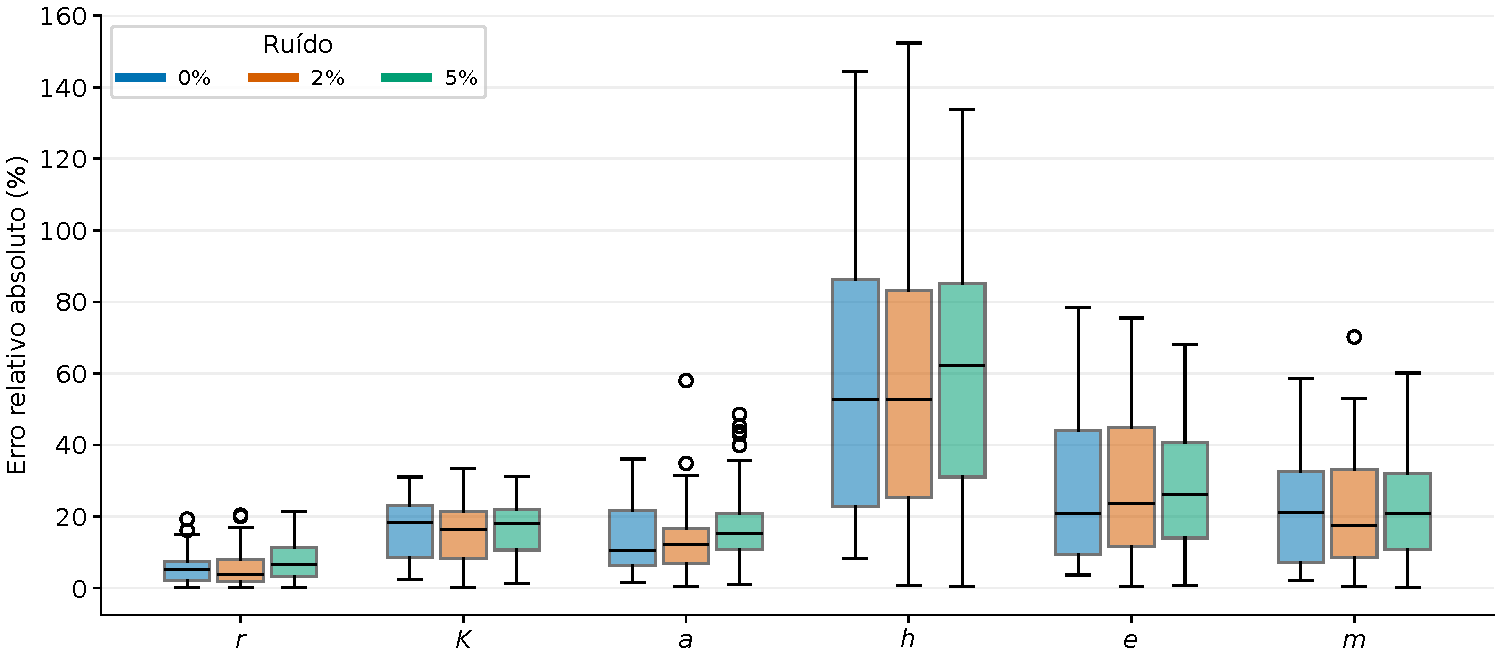
\includegraphics[width=\linewidth,height=0.76\textheight,keepaspectratio]{imgs/boxplot_erro_relativo_parametros.pdf}

  \smallskip
  \small Nos três níveis, $r$ teve o menor erro relativo absoluto médio
  (de $5{,}3\%$ a $7{,}3\%$) e $h$ teve o maior (de $56{,}1\%$ a $59{,}7\%$).
\end{frame}

\begin{frame}{Estimativas por execução sem ruído}
  \centering
  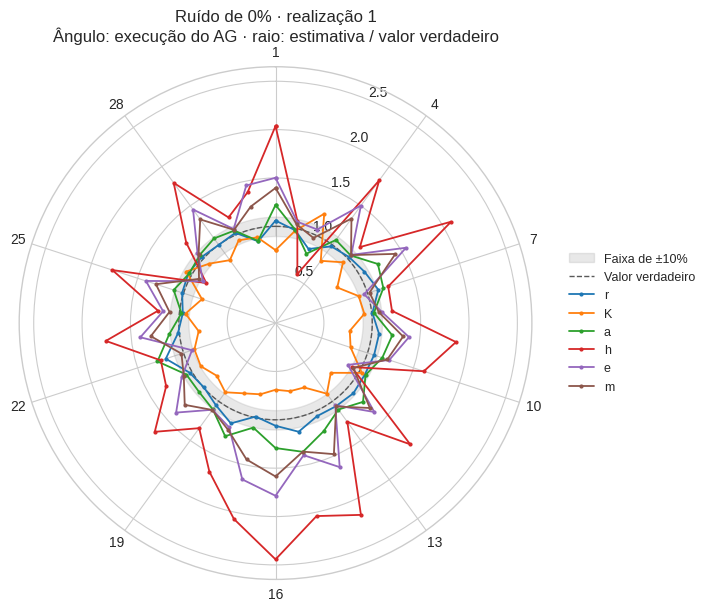
\includegraphics[height=0.9\textheight,keepaspectratio]{imgs/estimativas_execucao_ruido_00_realizacao_01.png}

\end{frame}

\begin{frame}{Estimativas por execução com ruído de 2\%}
  \centering
  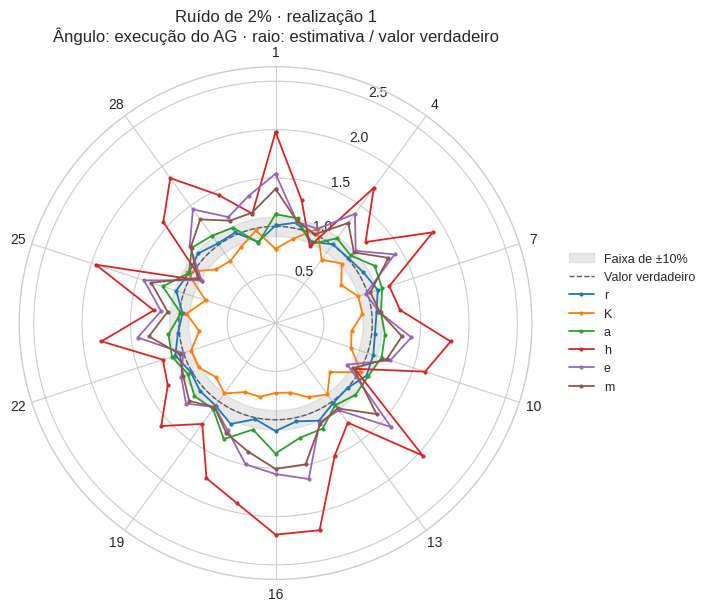
\includegraphics[width=0.325\linewidth]{imgs/estimativas_execucao_ruido_02_realizacao_01.png}\hfill
  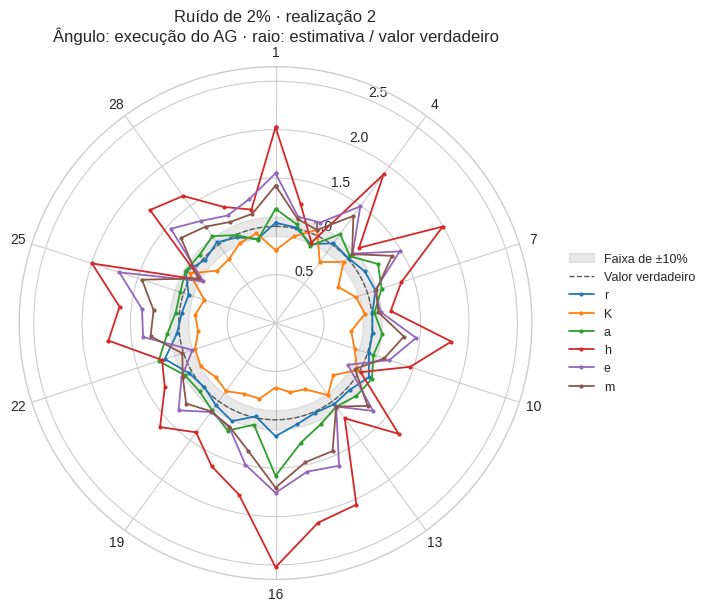
\includegraphics[width=0.325\linewidth]{imgs/estimativas_execucao_ruido_02_realizacao_02.png}\hfill
  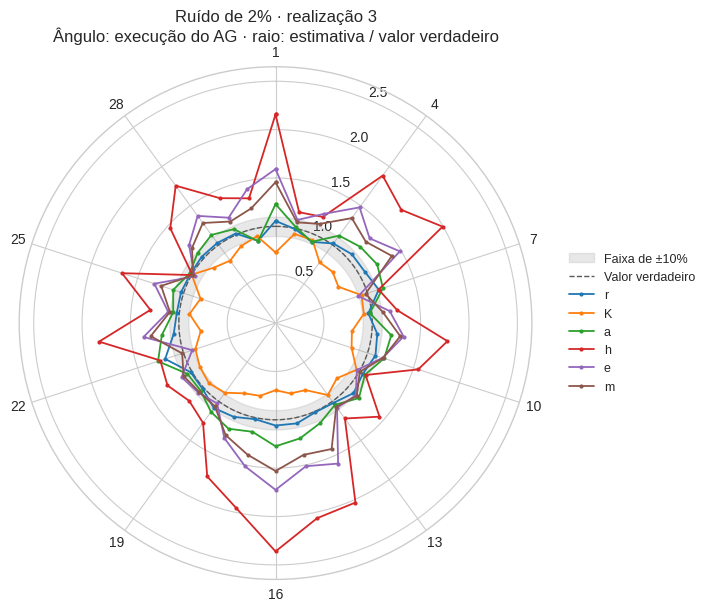
\includegraphics[width=0.325\linewidth]{imgs/estimativas_execucao_ruido_02_realizacao_03.png}

\end{frame}

\begin{frame}{Estimativas por execução com ruído de 5\%}
  \centering
  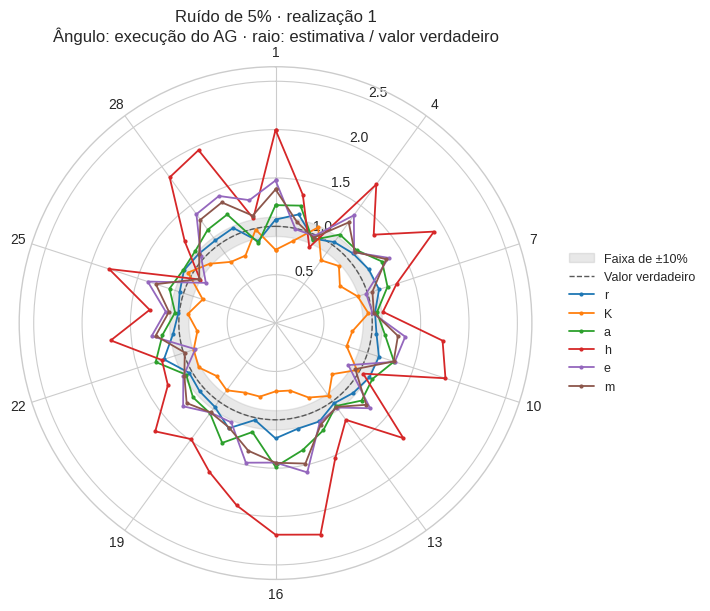
\includegraphics[width=0.325\linewidth]{imgs/estimativas_execucao_ruido_05_realizacao_01.png}\hfill
  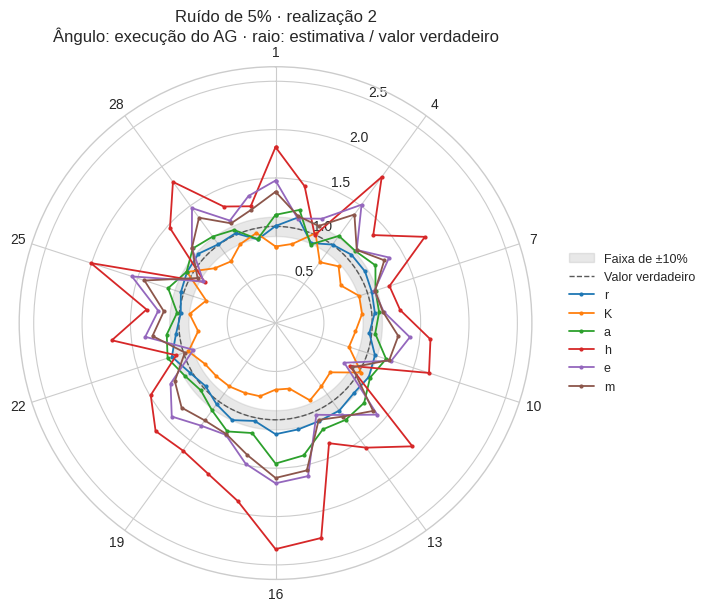
\includegraphics[width=0.325\linewidth]{imgs/estimativas_execucao_ruido_05_realizacao_02.png}\hfill
  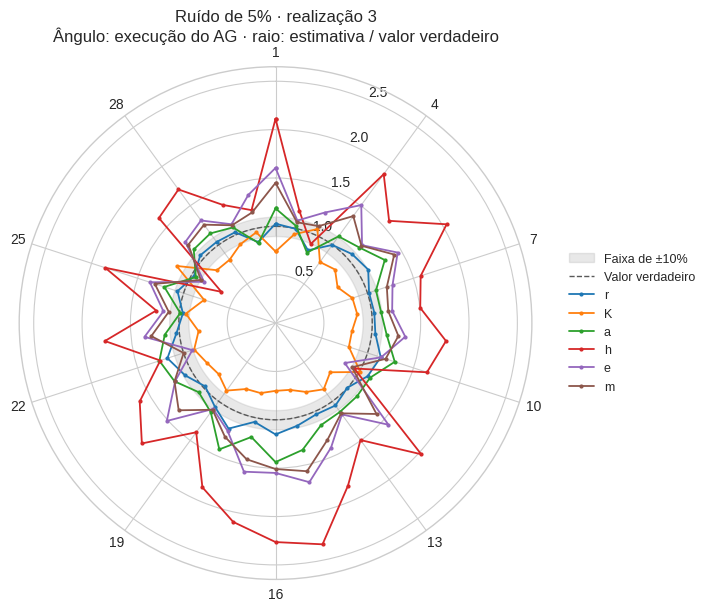
\includegraphics[width=0.325\linewidth]{imgs/estimativas_execucao_ruido_05_realizacao_03.png}
\end{frame}

\begin{frame}{Reconstrução das trajetórias de presas}
  \centering
  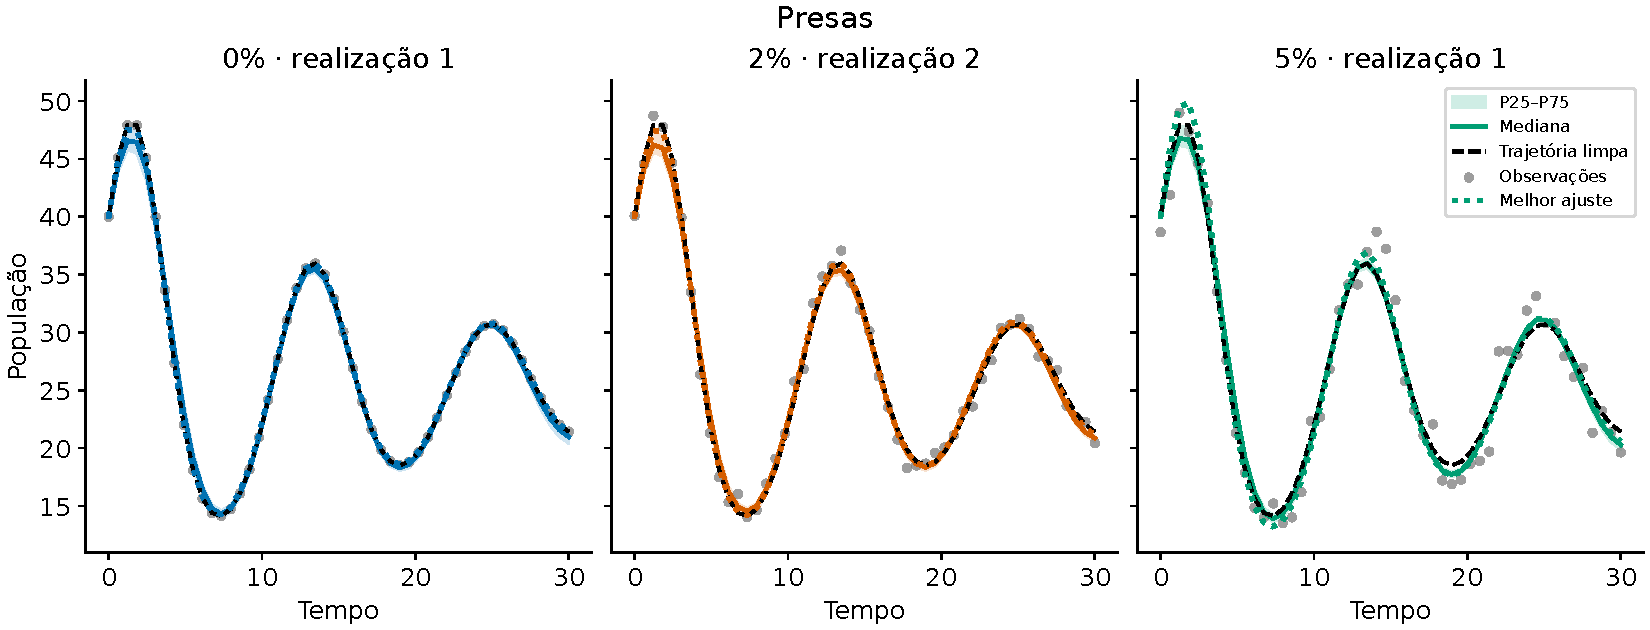
\includegraphics[width=\linewidth,height=0.76\textheight,keepaspectratio]{imgs/ajuste_representativo_presas.pdf}

\end{frame}

\begin{frame}{Reconstrução das trajetórias de predadores}
  \centering
  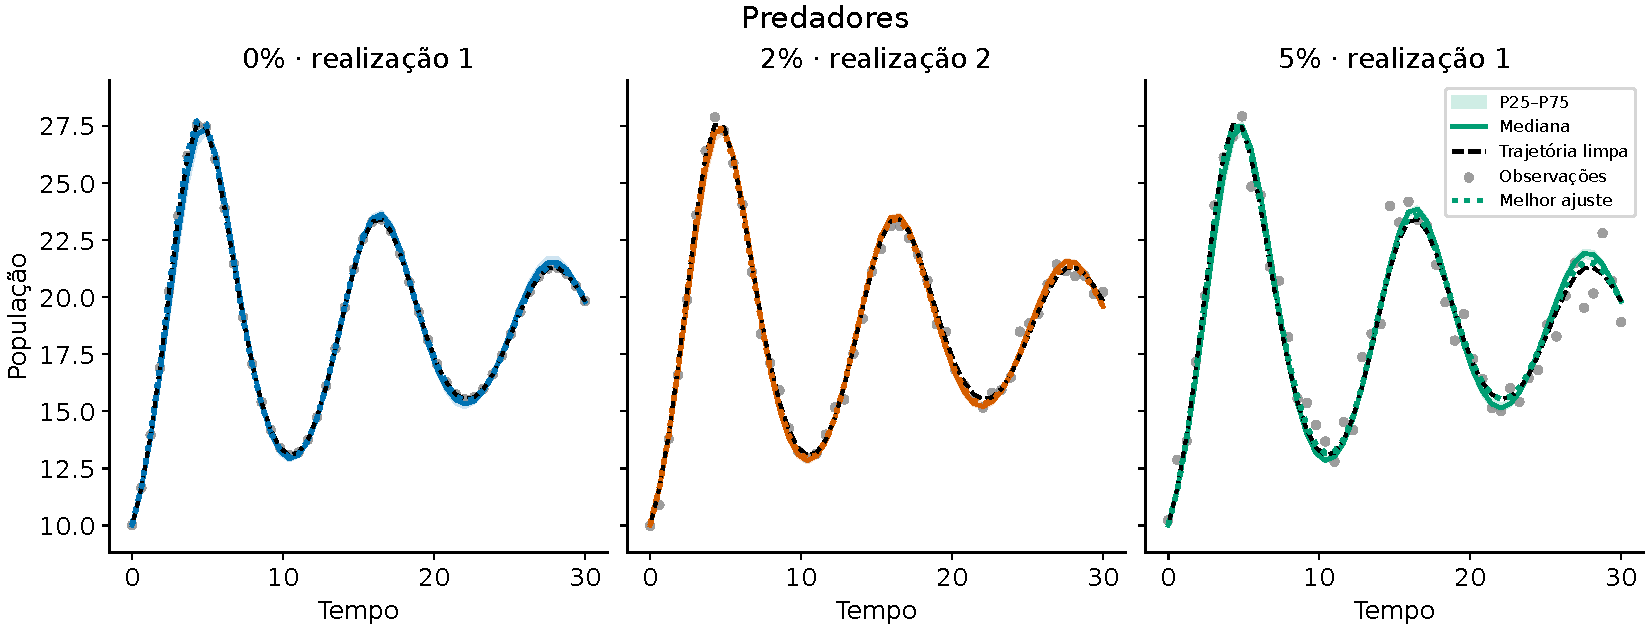
\includegraphics[width=\linewidth,height=0.76\textheight,keepaspectratio]{imgs/ajuste_representativo_predadores.pdf}

\end{frame}

\begin{frame}{Relação entre função objetivo e erro paramétrico}
  \centering
  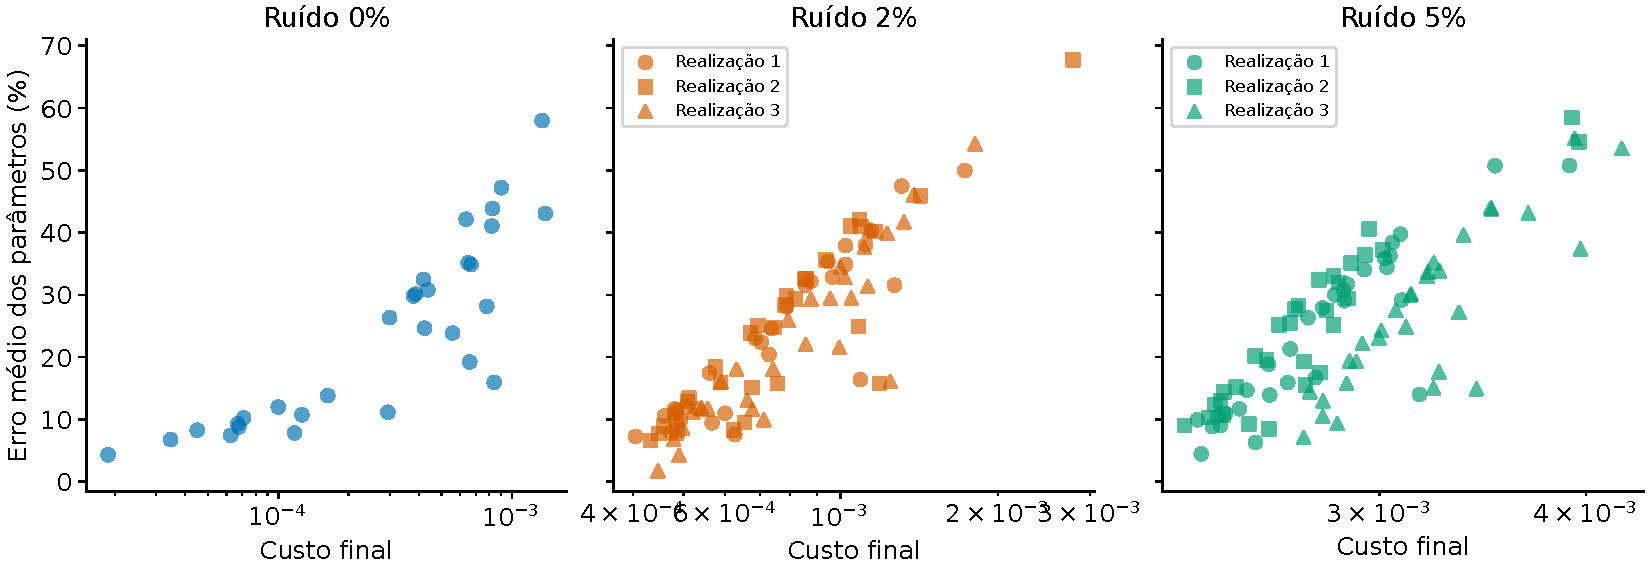
\includegraphics[width=\linewidth,height=0.76\textheight,keepaspectratio]{imgs/custo_final_vs_erro_parametros.pdf}

  \smallskip
  \small Das 56 execuções no quartil de menor custo em suas realizações,
  53 ficaram fora da tolerância em pelo menos um parâmetro.
  Em dados ruidosos, 17 de 180 estimativas tiveram $J(\hat{\theta})<J(\theta^*)$.
\end{frame}

\begin{frame}{Convergência do melhor custo}
  \centering
  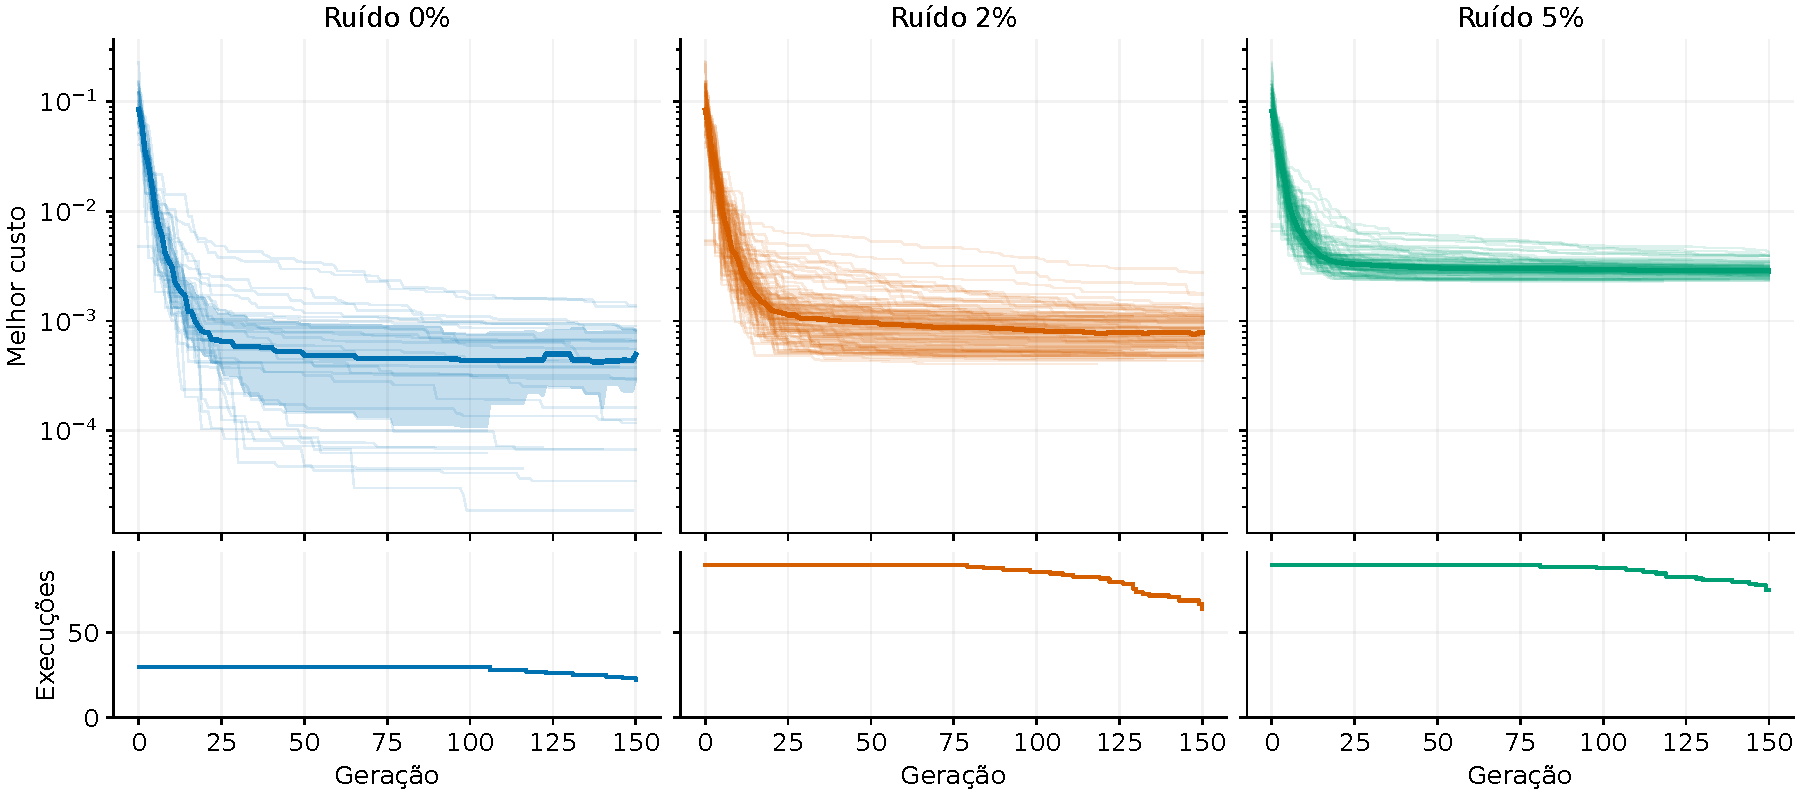
\includegraphics[width=\linewidth,height=0.76\textheight,keepaspectratio]{imgs/convergencia_melhor_custo.pdf}

  \smallskip
  \small Linhas finas mostram as execuções. A linha espessa e a faixa indicam
  mediana e P25--P75. O painel inferior conta apenas as execuções que chegaram
  a cada geração.
\end{frame}

\begin{frame}{Convergência do custo médio da população}
  \centering
  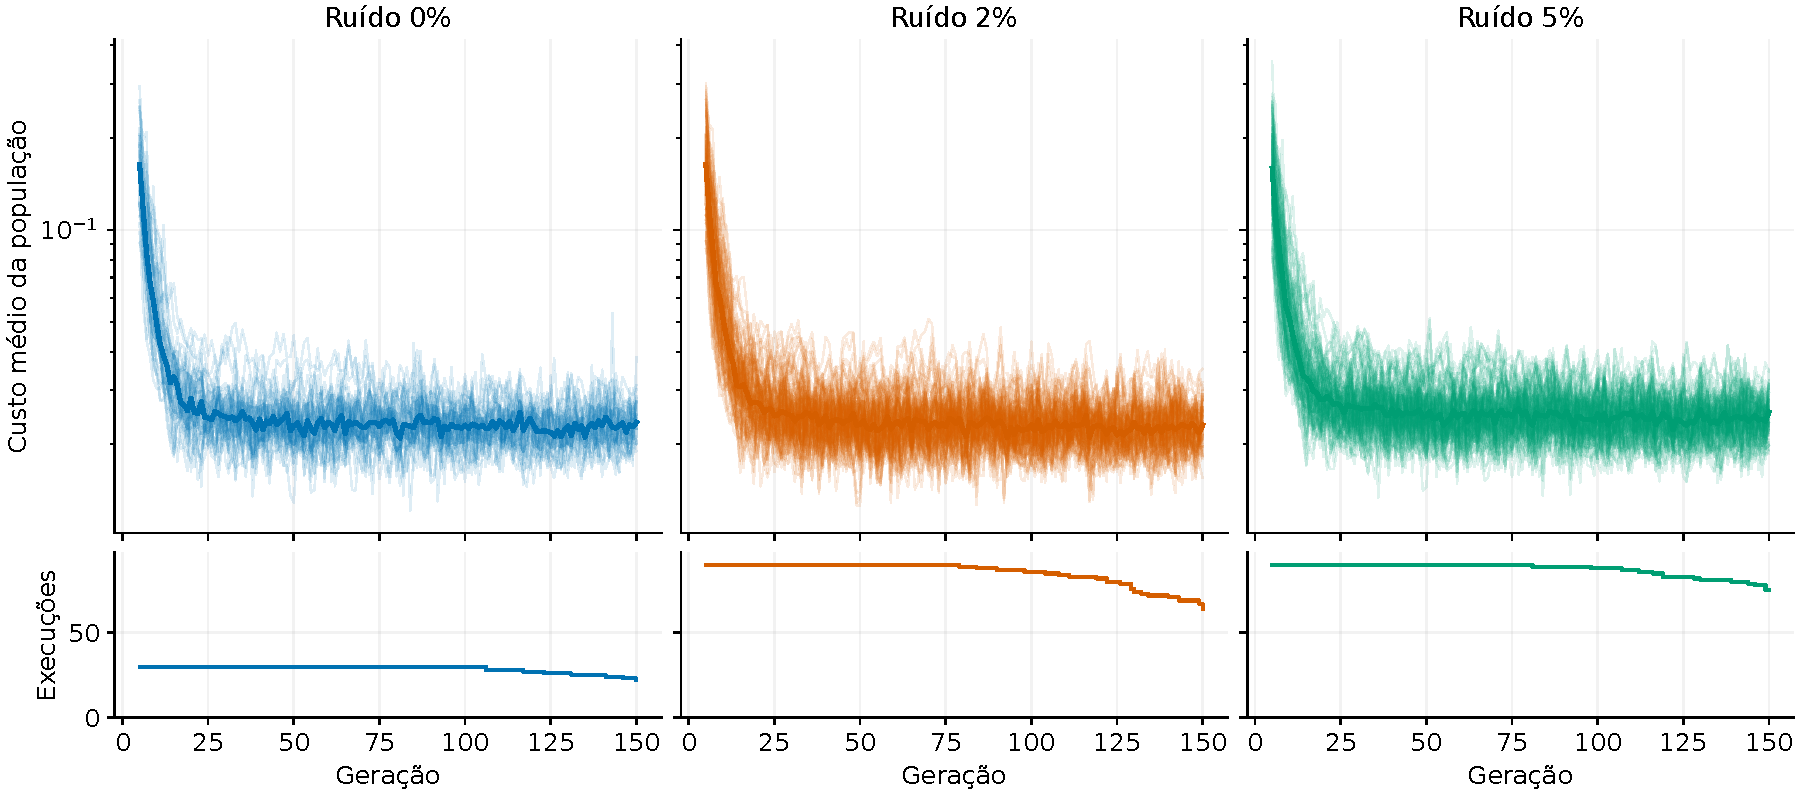
\includegraphics[width=\linewidth,height=0.76\textheight,keepaspectratio]{imgs/convergencia_custo_medio_apos_penalidades.pdf}

  \smallskip
  \small O recorte começa na geração 5, após o último sinal de penalidade.
  Depois da queda inicial, o custo médio oscila, enquanto o menor custo só pode
  diminuir ou permanecer constante pelo elitismo.
\end{frame}

\begin{frame}{Custo computacional e paradas antecipadas}
  \centering
  \begin{tabular}{lrrrr}
    \toprule
    Ruído & Tempo médio (s) & Avaliações médias & Geração final média & Paradas antecipadas \\
    \midrule
    $0\%$ & $159{,}0$ & 14\,042 & $143{,}7$ & $8/30$ \\
    $2\%$ & $157{,}7$ & 13\,921 & $142{,}5$ & $26/90$ \\
    $5\%$ & $158{,}9$ & 14\,242 & $145{,}8$ & $15/90$ \\
    \bottomrule
  \end{tabular}

  \medskip
  \begin{itemize}
    \item O total observado em cada execução é $100+97g$, com $g$ igual
          à geração final. O máximo é 14\,650 avaliações.
    \item Em 49 das 210 calibrações, a regra de 50 gerações sem melhora
          significativa disparou antes do limite de gerações.
  \end{itemize}
\end{frame}

\begin{frame}{Variabilidade entre realizações com ruído de 5\%}
  \centering
  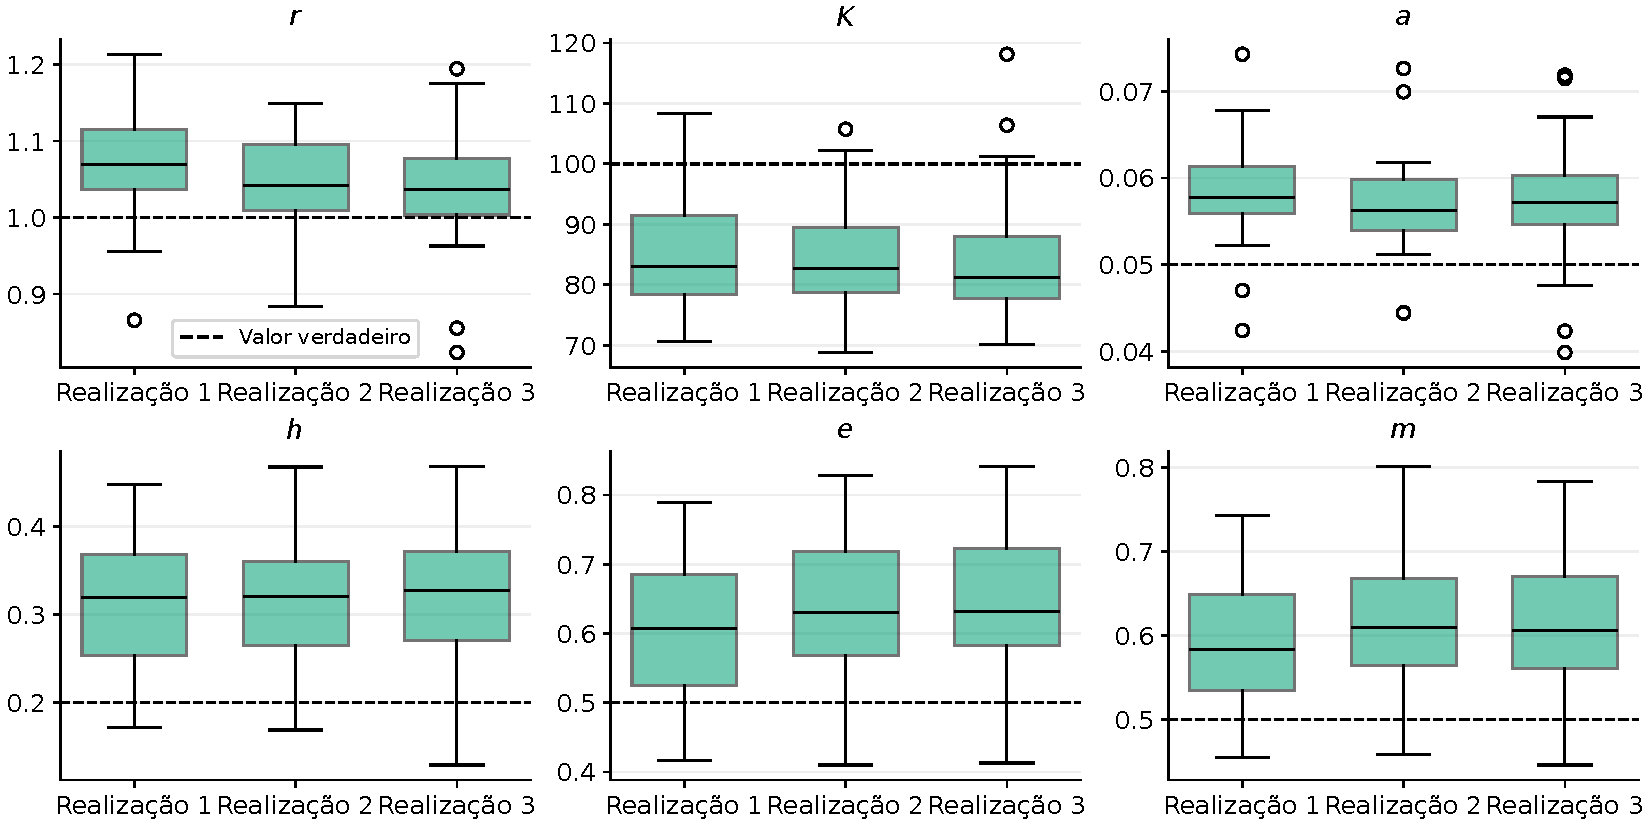
\includegraphics[width=\linewidth,height=0.76\textheight,keepaspectratio]{imgs/boxplot_por_realizacao_ruido_05.pdf}
\end{frame}

\section{Discussões}

\begin{frame}{Possíveis compensações entre parâmetros}
  \centering
  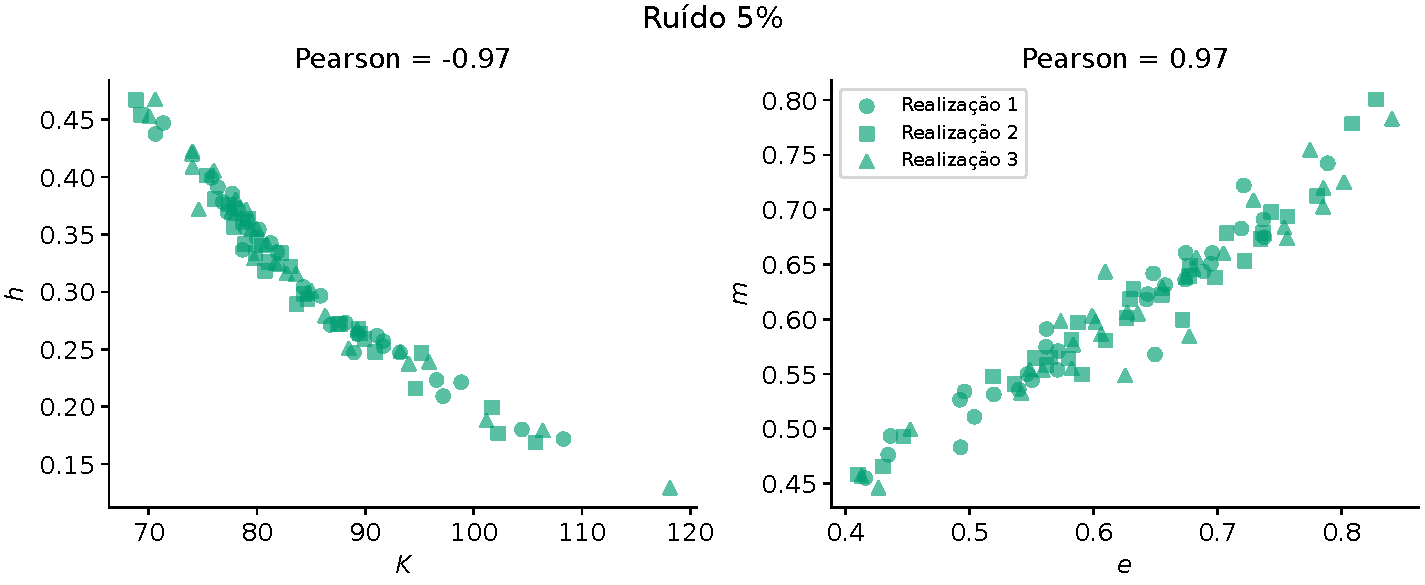
\includegraphics[width=\linewidth,height=0.76\textheight,keepaspectratio]{imgs/pares_correlacionados_ruido_05.pdf}

  \smallskip
  \small Com ruído de $5\%$, as correlações de Pearson entre os vencedores
  foram de $-0{,}97$ para $(K,h)$ e de $0{,}97$ para $(e,m)$.
  As associações são indícios de compensação, a investigar com uma análise
  de identificabilidade.
\end{frame}

\begin{frame}{Interpretação das compensações entre parâmetros}

  \textbf{Capacidade de suporte e tempo de manipulação:}
  \[
    \frac{dN}{dt}
    =
    rN\left(1-\frac{N}{K}\right)
    -\frac{aNP}{1+ahN}.
  \]

  \begin{itemize}
    \item O aumento de $K$ favorece o crescimento das presas.
    \item A redução de $h$ intensifica a predação.
    \item Possível compensação: $\rho_{K,h}=-0{,}97$.
  \end{itemize}

  \textbf{Eficiência de conversão e mortalidade:}
  \[
    \frac{dP}{dt}
    =
    e\frac{aNP}{1+ahN}-mP.
  \]

  \begin{itemize}
    \item O aumento de $e$ favorece o crescimento dos predadores.
    \item O aumento de $m$ intensifica a mortalidade.
    \item Possível compensação: $\rho_{e,m}=0{,}97$.
  \end{itemize}

\end{frame}

\begin{frame}{Possíveis problemas de identificabilidade}

  A identificabilidade está relacionada à capacidade de
  determinar os parâmetros de um modelo a partir das
  observações disponíveis.

  \medskip
  \textbf{Indícios observados neste trabalho:}

  \begin{itemize}
    \item Baixo erro na reconstrução das trajetórias, mesmo
          com elevados erros de estimação dos parâmetros.

    \item Dificuldade de recuperação dos parâmetros
          mesmo na ausência de ruído.

    \item Fortes correlações entre as estimativas de
          $(K,h)$ e $(e,m)$, sugerindo mecanismos
          de compensação.

    \item Diferentes conjuntos de parâmetros produzindo
          valores semelhantes da função objetivo.
  \end{itemize}

  \begin{block}{Hipótese}
    O problema pode apresentar dificuldades de
    identificabilidade prática, nas quais diferentes
    combinações de parâmetros produzem trajetórias
    semelhantes para as observações disponíveis.
  \end{block}

\end{frame}

\begin{frame}{SHAP: referência e vetores híbridos (em construção)}
  \begin{enumerate}
    \item Amostrar oito vetores por hipercubo latino na faixa de $\pm10\%$
          dos parâmetros verdadeiros, respeitando os limites de busca.
    \item Para uma estimativa $\hat\theta$ e um subconjunto $S$ dos seis
          parâmetros, manter os valores de $\hat\theta$ em $S$ e completar
          o vetor com cada uma das oito referências.
    \item Resolver as EDOs para os vetores híbridos e calcular a média dos
          custos $J$ contra as observações daquela realização. Essa média
          é $v(S)$.
  \end{enumerate}
\end{frame}

\begin{frame}{SHAP: contribuição dos parâmetros}
  O cálculo percorre os $2^6=64$ subconjuntos. Para o parâmetro $j$,
  $\phi_j$ é a média ponderada das mudanças
  $v(S\cup\{j\})-v(S)$ sobre os subconjuntos que ainda não contêm $j$.
  Os pesos equivalem a considerar todas as ordens de entrada dos parâmetros.
  \[
    J(\hat\theta)
    = \underbrace{v(\varnothing)}_{\text{custo médio da referência}}
      + \phi_r+\phi_K+\phi_a+\phi_h+\phi_e+\phi_m.
  \]

  \begin{itemize}
    \item Uma contribuição positiva aumenta o custo em relação à referência.
          Uma contribuição negativa o reduz.
    \item O gráfico usa a média de $|\phi_j|$ das 30 execuções de cada
          realização para comparar magnitudes sem cancelamento de sinais.
  \end{itemize}
\end{frame}

\begin{frame}{Contribuições SHAP para o custo de ajuste}
  \centering
  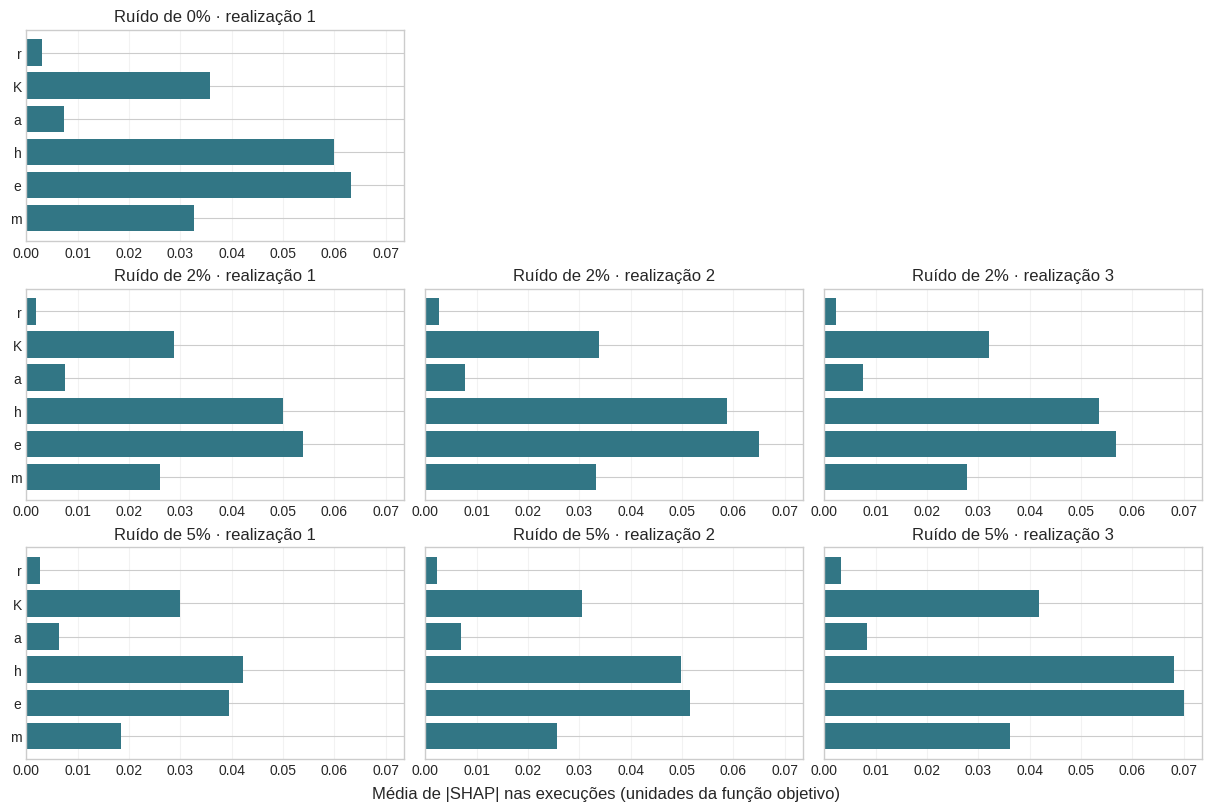
\includegraphics[width=\linewidth,height=0.9\textheight,keepaspectratio]{imgs/shap-por-cenario.png}
\end{frame}

\section{Conclusões}

\begin{frame}{Conclusões}

  \begin{itemize}
    \item O algoritmo genético apresentou boa capacidade de
          reconstrução das trajetórias populacionais, com
          NRMSE médio inferior a $2{,}5\%$ nos três níveis de ruído.

    \item A recuperação dos parâmetros mostrou-se mais difícil
          que o ajuste das trajetórias, inclusive na ausência
          de ruído.

    \item O parâmetro $r$ apresentou os menores erros de estimação,
          enquanto $h$ apresentou os maiores.

    \item As fortes correlações entre determinados parâmetros
          sugerem mecanismos de compensação na dinâmica do modelo.

    \item A introdução de ruído produziu uma variação relativamente
          pequena no erro paramétrico médio, nas condições avaliadas.
    
    \item A análise SHAP indicou que os parâmetros com maiores
      erros de estimação também apresentaram contribuições
      expressivas, em magnitude, para a função objetivo,
      sugerindo que os desvios em relação aos valores de
      referência exercem influência relevante sobre a
      qualidade do ajuste das trajetórias.
  \end{itemize}

  \begin{block}{Principal conclusão}
    Um bom ajuste das trajetórias populacionais não garante
    a recuperação precisa dos parâmetros do modelo.
  \end{block}

\end{frame}

\begin{frame}{Limitações e próximas etapas}
  \begin{itemize}
    \item O estudo usou um vetor verdadeiro e três realizações por nível ruidoso.
          Ampliar o protocolo para mais vetores e quantidades de observações.
    \item O arquivo de resultados guarda o vencedor de cada execução.
          Salvar as populações finais para medir diversidade e concentração nos limites.
    \item Usar diferentes discretizações e quantidade de observações.
    \item Exportar os valores SHAP individuais para analisar o sinal e a
          dispersão das contribuições por parâmetro.
    \item Investigar as compensações observadas e comparar o AG com a
          rede neural inversa e a PINN previstas na proposta.
  \end{itemize}
\end{frame}
